\documentclass[11pt]{article}
\usepackage[utf8]{inputenc}
\usepackage[a4paper,margin=0.8in]{geometry}
\usepackage{amsmath,hyperref,xurl,enumitem,titlesec,xcolor,fancyhdr,tikz,graphicx,eso-pic}
\graphicspath{{../}}
\definecolor{kcpc-text}{RGB}{20,20,20}
\definecolor{kcpc-muted}{RGB}{90,90,90}
\definecolor{kcpc-red}{RGB}{176,0,0}
\pagestyle{fancy}\fancyhf{}
\lhead{\textcolor{kcpc-text}{\small\bfseries Reading}}
\rhead{\textcolor{kcpc-muted}{\small Week 5}}
\cfoot{\textcolor{kcpc-muted}{\small KCPC}}
\renewcommand{\headrulewidth}{0.4pt}
\renewcommand{\headrule}{\hbox to\headwidth{\color{kcpc-red}\leaders\hrule height \headrulewidth\hfill}}
\renewcommand{\footrulewidth}{0pt}
\setlength{\headheight}{28pt}
\AddToShipoutPictureBG{\begin{tikzpicture}[remember picture,overlay]
  \node[opacity=0.035,at=(current page.center)]{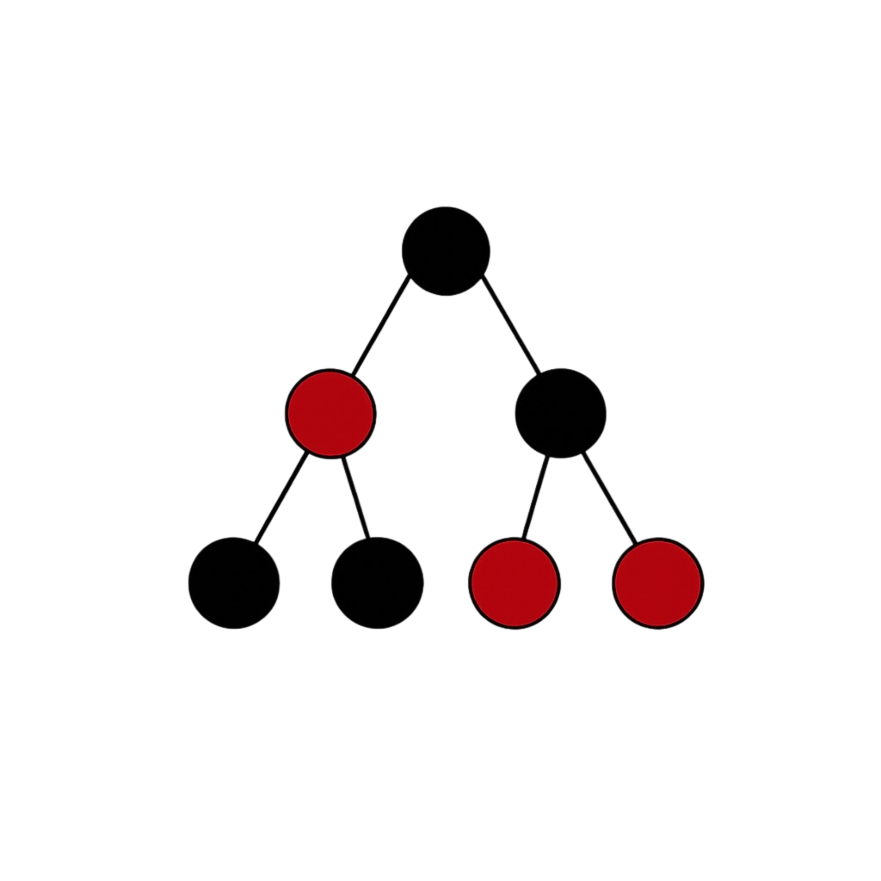
\includegraphics[width=0.38\paperwidth]{kcpc-logo.png}};
\end{tikzpicture}}
\titleformat{\section}{\large\bfseries\color{kcpc-red}}{}{0pt}{}
\setlist[itemize]{noitemsep,topsep=4pt}
\setlength{\parindent}{0pt}
\hypersetup{colorlinks=true,urlcolor=kcpc-red,linkcolor=kcpc-red}
\setlength{\emergencystretch}{1.5em}
\title{KCPC Week 5 Reading\\Graphs II: Dijkstra and 0--1 BFS}
\author{}\date{}

\begin{document}
\maketitle\thispagestyle{fancy}

Follow this guide alongside the slides and problem sheet. DFS and BFS are covered in \emph{Week 4 Reading}, which this workshop builds on, so this guide only adds what is new: priority queues, shortest paths with non-negative weights (Dijkstra), the relaxation invariant, and 0--1 BFS. For the original research behind these algorithms, see \emph{Week 5 Papers}.

\section*{I. Core algorithmic reading}
\subsection*{Guide to Competitive Programming (Antti Laaksonen-style community PDF)}
\url{https://duoblogger.github.io/assets/pdf/memonvyftw/guide-t-cp.pdf}
\begin{itemize}
  \item \textbf{Dijkstra's Algorithm, p.~89:} relaxation with a priority queue for non-negative weights; the basis for Problems 1--2, 4--5 and 9--15.
  \item \textbf{Bellman--Ford, p.~88 (further reading):} the negative-weight alternative the slides warn about; not required for this sheet.
  \item \textbf{Floyd--Warshall, p.~92 (further reading):} all-pairs shortest paths; optional context for why we only need single-source methods here.
\end{itemize}

\section*{II. 0--1 BFS}
\subsection*{CP-Algorithms}
\url{https://cp-algorithms.com/graph/01_bfs.html}

A concise explanation of 0--1 BFS, including its correctness argument and time complexity analysis. Read it before attempting the deque-based problems: 3 (arrow grid), 6 (obstacle removal), 8 (Wizard in Maze) and 15 (Stronger Takahashi). Compare its dial/bucket viewpoint with the slides' ``two adjacent distance levels'' invariant, and with Dial (1969) in \emph{Week 5 Papers}.

\section*{III. Formal textbook reference}
\subsection*{Introduction to Algorithms, 3rd Edition (Cormen, Leiserson, Rivest, Stein)}
\url{https://www.cs.mcgill.ca/~akroit/math/compsci/Cormen%20Introduction%20to%20Algorithms.pdf}

Page numbers below refer to the 3rd edition, as in \emph{Week 4 Reading}.
\begin{itemize}
  \item \textbf{Priority queues, p.~162 (\S6.5):} the heap operations behind the slides' lazy min-heap implementation.
  \item \textbf{Dijkstra's Algorithm, p.~658 (\S24.3):} the formal proof of the settling invariant the slides rely on, including why negative weights break it.
  \item \textbf{Bellman--Ford, p.~651 (\S24.1, further reading):} the correct tool when negative weights appear.
  \item \textbf{Floyd--Warshall, p.~693 (\S25.2, further reading):} optional all-pairs perspective.
\end{itemize}

\section*{Suggested order}
Start with the DFS and BFS reading in \emph{Week 4 Reading}. Then read the Dijkstra section of the competitive programming guide (p.~89) alongside the slides' worked traces, and solve Problems 1--3. Read the CP-Algorithms 0--1 BFS page, then attempt Problems 3, 6, 8 and 15. Use CLRS \S6.5 and \S24.3 for the heap operations and the formal settling invariant when writing up your own reasoning, and consult Bellman--Ford and Floyd--Warshall only as further reading. For original sources and historical context, see \emph{Week 5 Papers}.

\end{document}
